\documentclass[calculator,datasheet,handbook]{exam}
% The full list of class options are
% calculator : Allows approved calculator use.
% datasheet : Adds a note that data sheet are attached to the exam.
% handbook : Allows the use of the engineering handbook.
% resit : Adds the resit markings to the paper.
% sample : Adds conspicuous SAMPLE markings to the paper
% solutions : Uses the contents of \solution commands (and \solmarks) to generate a solution file
   
\usepackage{array}    
\usepackage{multirow}   
\usepackage{pdfpages}  
\usepackage[hidelinks]{hyperref}

\examtime{2~pm -- 5~pm}%
\examdate{13}{12}{2016}%
\examformat{Candidates should attempt \textit{all} questions.}

\newtoggle{3030paper}

%This changes the mode from EX3030 to EM40JN
\toggletrue{3030paper}
%\togglefalse{3030paper}

\iftoggle{3030paper}{
  \coursecode{EX3030}%
  \coursetitle{Heat, Mass, \& Momentum Transfer}%
}{
  \coursecode{EM40JN}%
  \coursetitle{Heat and Momentum Transfer}%
}

\begin{document}
%%%%%%%%%%%%%%%%%%%%%%%%%%%%%%%%%%%%%%%%%%%%%%%%%%%%%%%%%%%%%%%%%%%%%%%%%%%%%%%% 
%%%%%%%%%%%%%%%%%%%%%%%%%%%%%%%%%%%%%%%%%%%%%%%%%%%%%%%%%%%%%%%%%%%%%%%%%%%%%%%%

\begin{question}
  \begin{enumerate}[a)]
  \item Describe the physical interpretation of the Grashof number for
    natural convection. Describe each of its terms and write down an
    equation for the temperature at which temperature-dependent terms
    in Gr should be evaluated.%
    \marks{5}%
    \solution{%
      The Grashof number is the analogue of the Reynolds number for
      natural convection\solmarks{1} and is the ratio of bouyancy and viscous
      forces in the fluid.\solmarks{1} It is defined as
      \begin{align*}
        \text{Gr}=\frac{g\,\rho^2\,\beta\left(T_w-T_\infty\right)
        L^3}{\mu^2},
      \end{align*}
      where $g$ is the gravitational acceleration,\\*
      $\rho$ is the density of the fluid,\\*
      $\beta$ is the thermal expansion coefficient of the fluid,\solmarks{1}\\*
      $T_w$  is the wall temperature,\\*
      $T_\infty$ is the fluid temperature a large distance from the wall (bulk),\\*
      $L$ is a characterstic (and often vertical) length scale,\solmarks{1}\\*
      and $\mu$ is the fluid viscosity.
      
      The properties of the flow for the Grashof number should be
      evaluated at the so-called film temperature,
      \begin{align*}
        T_f &= \left(T_w+T_\infty\right) / 2
      \end{align*}\solmarks{1}
    }
  \item   An electric heater of 0.032~m diameter and 0.85~m in length is
    used to heat a room. Calculate the electrical input (i.e. the sum
    of heat transferred by convection and radiation) to the heater
    when the bulk of the air in the room is at 24${}^\circ$C, the
    walls are at 12${}^\circ$C, and the surface of the heater is at
    532${}^\circ$C. For convective heat transfer from the heater,
    assume the heater is a horizontal cylinder and the Nusselt number
    is given by
    \begin{align*}
      \text{Nu}=0.38(\text{Gr})^{0.25}
    \end{align*}
    where all properties are evaluated at the film temperature. You
    may assume air is an ideal gas, giving $\beta=T^{-1}$. Take the
    emissivity of the heater surface as ${\epsilon=0.62}$ and assume
    that the surroundings are black. All other properties should be
    calculated using the steam tables provided.\marks{10}%
    \solution{%
      Calculating the film temperature, we have
      \begin{align*}
        T_f = \frac{532 + 24}{2}=278^\circ\text{C}=551~\text{K}
      \end{align*}\solmarks{1}

      From the tables at 551~K, $\nu=4.48\times10^{-5}$~m${}^2$\,s${}^{-1}$ and
      $k=0.04375$~W\,m${}^{-1}$\,K${}^{-1}$. \solmarks{2} The expansion coefficient is
      $\beta=551^{-1}$~K${}^{-1}$\solmarks{1}. Combining these we have:
      \begin{align*}
        \text{Gr}=\frac{9.81\left(532 - 24\right)\,0.032^3}{551\left(4.48\times10^{-5}\right)^2} \approx 147\,700
      \end{align*}\solmarks{1}
      Calculating the Nusselt number, we have
      \begin{align*}
        \text{Nu}=0.38\left(147\,700\right)^{1/4}\approx 7.45 
      \end{align*}\solmarks{1}
      Calculating the convective coefficient we have
      \begin{align*}
        h = \frac{k\,Nu}{L}=\frac{0.04375\times7.45}{0.032}\approx 10.19\text{W}\,\text{m}^{-2}\,\text{K}^{-1}
      \end{align*}\solmarks{1}
      Heat transfer via convection:
      \begin{align*}
        Q_{conv} = h\,A\,\Delta T = 10.19\times\pi\times0.032\times0.85\left(532-24\right) \approx 442 \text{W}
      \end{align*}\solmarks{1}
      Heat transfer by radiation
      \begin{align*}
        Q_{rad.} &=\sigma\,\epsilon\,A\,\left(T_w^4 - T_\infty^4\right)\\
                 &=5.67\times10^{-8}\times0.62\times\pi\times0.032\times0.85\left(805^4-285^4\right)\\
                 &\approx 1242
      \end{align*}\solmarks{1}
      Total energy input is
      \begin{align*}
        Q_{total}=Q_{rad.} + Q_{conv}= 1242+442 = 1684~\text{W}
      \end{align*}\solmarks{1}
    }
  \item Using index notation, prove the following vector calculus identity:
    \begin{align*}
      \nabla^2\,f\,g = f\,\nabla^2\,g + 2(\nabla\,f)\cdot(\nabla\,g) + g\,\nabla^2\,f
    \end{align*}\marks{5}

    {\bf Note:} You must treat $f$ and $g$ as functions of $x,y,z$.
    \solution{%
      Converting to index notation in Cartesian coordinates (x,y,z),
      \begin{align*}
        \nabla^2\,f\,g = \frac{\partial}{\partial r_i} \left(\frac{\partial}{\partial r_i}\,f\,g\right)
      \end{align*}\solmarks{1}
      We can't use $\partial^2/\partial r_i^2$ as there is no repeated
      $i$ index. Using the product rule on the term in parenthesis
      \begin{align*}
        \frac{\partial}{\partial r_i}\,f\,g = f\frac{\partial g}{\partial r_i} + g\frac{\partial f}{\partial r_i}
      \end{align*}\solmarks{1}
      Using the product rule again to apply the second derivative to both of these terms gives
      \begin{align*}
        \frac{\partial}{\partial r_i}\frac{\partial}{\partial r_i}\,f\,g 
        &= \frac{\partial f}{\partial r_i}\frac{\partial g}{\partial r_i} + f\frac{\partial}{\partial r_i}\frac{\partial g}{\partial r_i} + \frac{\partial g}{\partial r_i}\frac{\partial f}{\partial r_i} +g \frac{\partial}{\partial r_i}\frac{\partial f}{\partial r_i}\\
        &=f\frac{\partial}{\partial r_i}\frac{\partial g}{\partial r_i} +2\frac{\partial f}{\partial r_i}\frac{\partial g}{\partial r_i} + g \frac{\partial}{\partial r_i}\frac{\partial f}{\partial r_i}
      \end{align*}\solmarks{2}
      Converting back to vector notation, yields the identity,
      \begin{align*}
        \frac{\partial}{\partial r_i}\frac{\partial}{\partial r_i}\,f\,g 
        &= f\,\nabla^2\,g + 2(\nabla\,f)\cdot(\nabla\,g) + g\,\nabla^2\,f
      \end{align*}\solmarks{1}
    }
  \end{enumerate}
\end{question}

\pagebreak
\begin{question}
  A wire-coating die consists of a cylindrical wire of radius,
  $\kappa\,R$, moving horizontally at a constant velocity, $v_{wire}$,
  along the axis of a cylindrical die of radius, $R$. You may assume
  the pressure is constant within the die (it is not pressure driven
  flow) but the flow is driven by the motion of the wire (it is
  ``axial annular Couette flow''). Neglect end effects and assume an
  isothermal system.
  \begin{figure}[ht]%
    \begin{center}%
      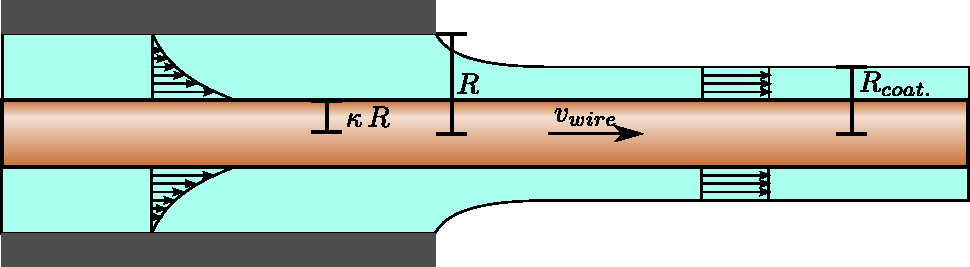
\includegraphics[width=0.8\linewidth,clip]{figures/wire_coating_die}%
    \end{center}
    \caption{\label{fig:wire_coating} Diagram of a wire coating die.}
  \end{figure}
  \begin{enumerate}[a)]
  \item State the two relevant boundary conditions for the flow within
    the die and how they arise. \marks{2} \solution{%
      Both conditions arise from non-slip conditions of the fluid with
      a solid boundary.\solmarks{1}
      
      \begin{itemize}
      \item $v_z(r=R)=0$: At the die wall interface.
      \item $v_z(r=\kappa\,R)=v_{wire}$: At the wire interface.
      \end{itemize}\solmarks{1}
    }
  \item The stress profile for an annular system is of the following
    form
    \begin{align*}
      \frac{1}{r}\frac{\partial}{\partial r} r\,\tau_{rz} = -\frac{\partial p}{\partial z}+\rho\,g_z.
    \end{align*}
    Derive the following expression for the flow profile
    \begin{align*}
      v_z = \frac{v_{wire}}{\ln \kappa}\ln\left(\frac{r}{R}\right).
    \end{align*}\marks{9}
    \solution{%
      There is no driving pressure gradient, and as the flow is
      horizontal, the two terms on the right hand side are zero
      \begin{align*}
        \frac{1}{r}\frac{\partial}{\partial r} r\,\tau_{rz} = -\cancelto{0}{\frac{\partial p}{\partial z}}+\rho\,\cancelto{0}{g_z}.
      \end{align*}\solmarks{2}

      Performing the integration of the stress profile expression from
      the previous question,
      \begin{align*}
        \tau_{rz} = \frac{C_1}{r}.
      \end{align*}\solmarks{1}
      
      Assuming the fluid is Newtonian, we have
      \begin{align*}
        -\mu \frac{\partial v_z}{\partial r} = \frac{C_1}{r}.
      \end{align*}\solmarks{1}

      Performing the integration
      \begin{align*}
        v_z = -\mu^{-1}\,C_1\ln\,r+C_2.
      \end{align*}\solmarks{1}
      
      Inserting the two boundary conditions yields the following
      \begin{align*}
        0 &= -\mu^{-1}\,C_1\ln R+C_2.\\
        v_{wire} &= -\mu^{-1}\,C_1\ln \kappa\,R+C_2.\\
      \end{align*}\solmarks{1}

      Solving both equations for the constants,
      \begin{align*}
        C_2 &= \mu^{-1}\,C_1\ln R\\
        v_{wire} &= \mu^{-1}\,C_1(\ln R-\ln \kappa\,R)\\
        C_1 &= -\frac{\mu\,v_{wire}}{\ln \kappa}.\\
      \end{align*}\solmarks{2}

      Inserting these back in gives the final expression
      \begin{align*}
        v_z = \frac{v_{wire}}{\ln \kappa}\ln\left(\frac{r}{R}\right)
      \end{align*}\solmarks{1}
    } 
  \item Derive the following expression for the volumetric flow-rate of liquid
    through the die
    \begin{align*}
      \dot{V}_z &= -\pi\,R^2\,v_{wire}\left({\kappa^2}+\frac{1-\kappa^2}{2\ln \kappa}\right).
    \end{align*}
    \marks{5}
    \\{\bf Note:} You will need the integration identity
    \begin{align*}
      \int x\,\ln(x)\,{\rm d}x = \frac{x^2}{2}\left(\ln(x) - \frac{1}{2}\right).
    \end{align*}
    \solution{%
      To determine the volumetric flow rate, the following integration is performed
      \begin{align*}
        \dot{V}_z = 2\,\pi\,\int_{\kappa\,R}^R r\,v_z\,{\rm d}r
      \end{align*}\solmarks{1}
      
      Performing the integration
      \begin{align*}
        \dot{V}_z &= 2\,\pi\,R\frac{v_{wire}}{\ln \kappa}\int_{\kappa\,R}^R \frac{r}{R}\ln\left(\frac{r}{R}\right){\rm d}r\\
                  &= \frac{2\,\pi\,R^2\,v_{wire}}{\ln \kappa}\int_{\kappa}^1 x\,\ln\left(x\right){\rm d}x\\
                  &= \frac{2\,\pi\,R^2\,v_{wire}}{\ln \kappa}\left[\frac{x^2}{2}\left(\ln x - \frac{1}{2}\right)\right]^1_{\kappa}\\
                  &= -\frac{2\,\pi\,R^2\,v_{wire}}{\ln \kappa}\left(\frac{\kappa^2}{2}\left(\ln \kappa - \frac{1}{2}\right) +\frac{1}{4}\right)\\
                  &= -\pi\,R^2\,v_{wire}\left({\kappa^2}+\frac{1-\kappa^2}{2\ln \kappa}\right)
      \end{align*}\solmarks{4}
    }
  \item Derive an expression for the outer radius of the coating,
    $R_{coat.}$, far away from the die exit. \marks{4} \solution{%
      Solving the stress balance again but for the film coating the
      wire, the following expression is found again for the stress
      \begin{align*}
        \tau_{rz} = \frac{C_1}{r}
      \end{align*}  
      At the exposed surface of the film ($r\neq0$), the stress is
      zero (assuming the air exerts close to zero drag). This implies
      that $C_1=0$ as well, as it is the only possible way to set the
      RHS to zero at finite values of $r$. As the stress is zero,
      Newton's law of viscosity then implies the film has a constant
      velocity which will be the velocity of the wire (note, the
      diagram gives the student a strong hint that this is
      true).\solmarks{2}
      
      The volumetric flowrate of the wire coating is related to the
      outer radius of the coating, $R_{coat.}$
      \begin{align*}
        \dot{V}_{z,coating}=v_{wire}\,\pi\left(R_{coat.}^2-\kappa^2\,R^2\right)
      \end{align*}\solmarks{1}
      This must be equal to the volumetric flowrate of coating through the die
      \begin{align*}
        v_{wire}\,\pi\left(R_{coating}^2-\kappa^2\,R^2\right)
        &= -\pi\,R^2\,v_{wire}\left({\kappa^2}+\frac{1-\kappa^2}{2\ln \kappa}\right)\\
        R_{coating}
        &=R\sqrt{\frac{\kappa^2-1}{2\ln \kappa}}
      \end{align*}\solmarks{1}
    }
  \end{enumerate}
\end{question}


\begin{question}
  % Question 10B.4 pg 322 Transport Phenomena 2nd Ed.
  To explore the effect of using a temperature-dependent thermal
  conductivity, consider heat flowing through an annular (pipe) wall
  of inside radius $R_{0}$ and an outside radius $R_{1}$. It is
  assumed that thermal conductivity varies linearly with temperature
  from $k_{0}(T=T_{0})$ to $k_{1}(T=T_{1})$ where $T_{0}$ and $T_{1}$
  are the inner and outer wall temperatures respectively.
  \begin{figure}[ht]%
    \begin{center}%
      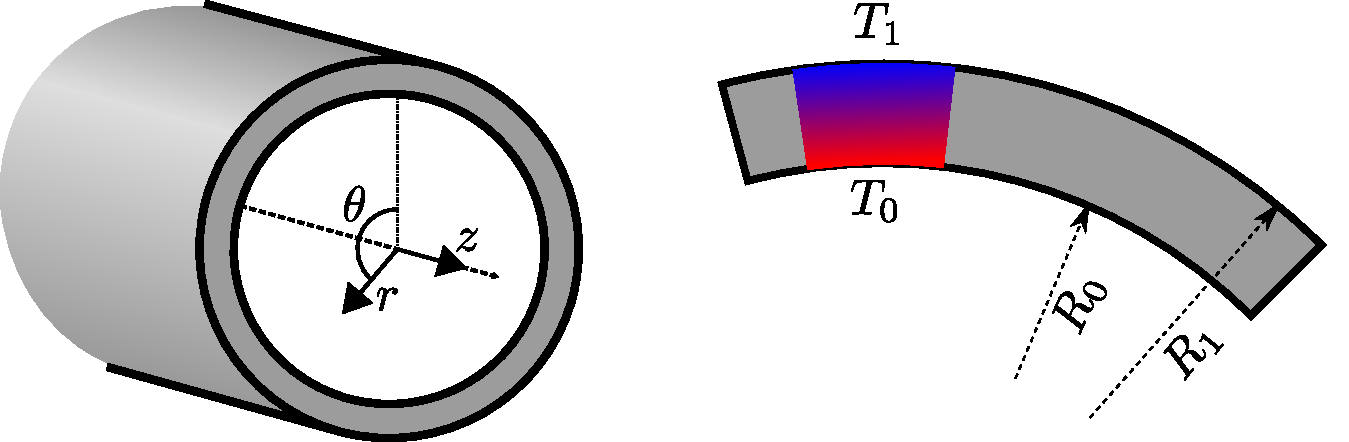
\includegraphics[width=0.8\linewidth,clip]{figures/cyl_cond}%
    \end{center}
    \caption{\label{fig:cylindrical_cond} Conduction through an annular(pipe) wall.}
  \end{figure}
  \begin{enumerate}[a)]
  \item Derive the following energy balance equation
    \begin{align*}
      \frac{\partial}{\partial r} r\, q_r &= 0,
    \end{align*}
    and state ALL assumptions required.\marks{7}
    \solution{%
      Assuming that the pressure dependency of the internal energy of
      the solid is small\solmarks{1}, \autoref{eq:energybalance} can
      be used valid.

      As this is heat transfer in solids, we can set the frame of
      reference to the wall and $\bm{v}=\bm{0}$.  This greatly
      simplifies the energy balance equation:
      \begin{align*}
        \rho\,C_p\frac{\partial T}{\partial t} =& -\cancelto{0}{\rho\,C_p\, v_j
                                                  \,\nabla_j\,T} - \nabla_i\,q_i - \cancelto{0}{\tau_{ji}\,\nabla_j\,v_i} -
                                                  \cancelto{0}{p\,\nabla_i\,v_i} +\sigma_{energy}\\
        \rho\,C_p\frac{\partial T}{\partial t} =& - \nabla_i\,q_i +\sigma_{energy}
      \end{align*}\solmarks{1}
      
      Assuming the wall does not generate heat:
      \begin{align*}
        \rho\,C_p\frac{\partial T}{\partial t} =& - \nabla_i\,q_i +\cancelto{0}{\sigma_{energy}}
      \end{align*}\solmarks{1}

      And steady state:
      \begin{align*}
        \cancelto{0}{\rho\,C_p\frac{\partial T}{\partial t}} =& - \nabla_i\,q_i\\
        \nabla_i\,q_i = 0
      \end{align*}\solmarks{1}

      Finally, inserting the cylindrical coordinate system definition
      of $\nabla_i\,q_i$:
      \begin{align*}
        \nabla_i\,q_i &= \frac{1}{r}\frac{\partial}{\partial r}\left(r\,
                        q_r\right) + \frac{1}{r}\frac{\partial\,q_\theta}{\partial
                        \theta}+ \frac{\partial\,q_z}{\partial z}
      \end{align*}\solmarks{2}
      Assuming a symmetry of the system ALONG and AROUND the axis, the
      only remaining derivative is in the $r$-direction:
      \begin{align*}
        \nabla_i\,q_i &= \frac{1}{r}\frac{\partial}{\partial r}\left(r\,
                        q_r\right)\\
                      &= \frac{\partial}{\partial r}\left(r\,
                        q_r\right)=0
      \end{align*}\solmarks{1}
      As required.
    }
  \item Derive the following expression for the temperature profile
    \begin{align*}
      Q_r &= \frac{2\pi\,L}{{\ln\left(\frac{R_{0}}{R_{1}}\right)}}\frac{k_{1}+k_{0}}{2}(T_{1}-T_{0}),
    \end{align*}
    where $L$ is the length of the pipe/annulus.\marks{10}\\
    {\bf Note:} You will need the following identity:
    \begin{align*}
      T_{1}^2-T_{0}^2=(T_{1}+T_{0})(T_{1}-T_{0}).
    \end{align*}
    \solution{%
      Performing the integration, we have
      \begin{align*}
        r\, q_r &= C_1\\
        q_r &= \frac{C_1}{r}
      \end{align*}\solmarks{1}
      Inserting in Fourier's law, we have
      \begin{align*}
        -k \frac{\partial T}{\partial r} &= \frac{C_1}{r}
      \end{align*}
      We need to insert the temperature dependent thermal
      conductivity, which is given by the following linear relationship
      \begin{align*}
        k = k_{0} + \left(T-T_{0}\right)\frac{k_{1}-k_{0}}{T_{1}-T_{0}}
      \end{align*}\solmarks{1}
      Inserting this,
      \begin{align*}
        -\left(k_{0} + \left(T-T_{0}\right)\frac{k_{1}-k_{0}}{T_{1}-T_{0}}\right) \frac{\partial T}{\partial r} &= \frac{C_1}{r}
      \end{align*}\solmarks{1}
      Integrating between the two limits,
      \begin{align*}
        -\int_{R_{0}}^{R_{1}}\left(k_{0} + \left(T-T_{0}\right)\frac{k_{1}-k_{0}}{T_{1}-T_{0}}\right) \frac{\partial T}{\partial r}{\rm d}r&= \int_{R_{0}}^{R_{1}}\frac{C_1}{r}{\rm d}r\\
        -\int_{T_{0}}^{T_{1}}\left(k_{0} + \left(T-T_{0}\right)\frac{k_{1}-k_{0}}{T_{1}-T_{0}}\right){\rm d}T&= C_1\ln\left(\frac{R_{1}}{R_{0}}\right)\\
        -\left(k_{0}\left(T_{1}-T_{0}\right) + \left(\frac{T_{1}^2-T_{0}^2}{2}-\left(T_{1}-T_{0}\right)T_{0}\right)\frac{k_{1}-k_{0}}{T_{1}-T_{0}}\right)&= C_1\ln\left(\frac{R_{1}}{R_{0}}\right)
      \end{align*}\solmarks{2}
      Using the identity $T_{1}^2-T_{0}^2=(T_{1}+T_{0})(T_{1}-T_{0})$,
      \begin{align*}
        -\left(k_{0}\left(T_{1}-T_{0}\right) + \frac{T_{1}+T_{0}}{2}(k_{1}-k_{0})-T_{0}(k_{1}-k_{0})\right)&= C_1\ln\left(\frac{R_{1}}{R_{0}}\right)\\
        -\left(k_{0}\,T_{1} + \frac{T_{1}+T_{0}}{2}(k_{1}-k_{0})-T_{0}\,k_{1}\right)&= C_1\ln\left(\frac{R_{1}}{R_{0}}\right)
      \end{align*}\solmarks{2}
      Simple cancellation and factorisation leads to the following
      \begin{align*}
        \frac{k_{1}+k_{0}}{2\ln\left(\frac{R_{0}}{R_{1}}\right)}(T_{1}-T_{0})&= C_1
      \end{align*}\solmarks{1}
      Inserting this back into the expression for the flux, we have
      \begin{align*}
        q_r &= \frac{C_1}{r}\\
            &= \frac{k_{1}+k_{0}}{2\,r\ln\left(\frac{R_{0}}{R_{1}}\right)}(T_{1}-T_{0})
      \end{align*}\solmarks{1}
      The total flux is given by multiplying by the cylindrical area, $2\,\pi\,r\,L$,
      \begin{align*}
        Q_r &= \frac{2\pi\,L}{{\ln\left(\frac{R_{0}}{R_{1}}\right)}}\frac{k_{1}+k_{0}}{2}(T_{1}-T_{0})            
      \end{align*}\solmarks{1}
    }
  \item Compare this expression to the standard expression for
    conduction in pipe walls (with constant thermal conductivity),
    what can you observe? \marks{3}%
    \solution{%
      The expression for pipes is availabe from the tables in the
      datasheet, and is as follows
      \begin{align*}
        Q = \frac{2\pi\,L\,k}{\ln\left(\frac{R_{1}}{R_{0}}\right)}\Delta T.
      \end{align*}\solmarks{1}

      On comparision with the derived equation, the only change is to
      replace the constant thermal conductivity with the average of
      the thermal conductivity on the inner and outer
      surfaces. \solmarks{1}

      For \underline{small} temperature differences (where a linear
      temperature dependence may be assumed) using the average thermal
      conductivity is a useful strategy.\solmarks{1}
      
    }
  \end{enumerate}
\end{question}

\pagebreak
\iftoggle{3030paper}{
  \begin{question}
    To maintain a pressure close to 1~atm, an industrial pipeline
    containing ammonia gas is vented to ambient air.  Venting is
    achieved by tapping the pipe and inserting a 3~mm diameter tube,
    which extends for 20~m into the atmosphere.  With the entire system
    operating at 25$^\circ$C and 1 bar, the ideal gas equation of state
    predicts a total molar concentration of 40.9~mol/m${}^3$.  Equimolar
    counter-diffusion can be assumed, and both the concentration of air
    in the pipeline and the concentration of ammonia in the atmosphere
    can be considered negligible.  The diffusion coefficient of ammonia
    through air is approximately $2\times10^{-5}$~m$^2$/s.
    \begin{enumerate}[a)]
    \item Determine the mass rate of ammonia lost in to the atmosphere
      ${\bf N}_A$ in kg/h and the mass rate of contamination of the pipe
      with air ${\bf N}_B$ in the same units. \marks{12}

      \solution{%
        There is no generation of mass in the flow, and the system is at
        steady state\solmarks{1}, thus
        \begin{align*}
          \cancelto{0}{\frac{\partial C_A}{\partial t}} &= -\nabla\cdot\bm{N}_{A} + \cancelto{0}{\sigma_A}\\
          \nabla\cdot\bm{N}_{A} &= 0
        \end{align*}
        Using rectangular coordinates, and treating this as a one
        dimensional flow we find that the fluxes of the ammonia and air
        are constant.\solmarks{1}
        \begin{align*}
          \frac{\partial N_{A,x}}{\partial x} &= 0
        \end{align*}      
        Thus,
        \begin{align*}
          N_{A,z} &= N_{A,0} & N_{B,z} &= N_{B,0}
        \end{align*}
        The boundary conditions are
        \begin{align*}
          C_A(z=0~\text{m})&=40.9~{\rm mol/m}^3 & C_A(z=20~\text{m})&=0~{\rm mol/m}^3\\
          C_B(z=0~\text{m})&=0~{\rm mol/m}^3 & C_B(z=20~\text{m})&=40.9~{\rm mol/m}^3
        \end{align*}\solmarks{2}
        If the system is an ideal gas, and there is no pressure driven
        flow (assumed by the pipeline being at 1~atm), this is equimolar
        counterdiffusion\solmarks{2}, thus $N_{B,0}=-N_{A,0}$.  

        For equimolar counterdiffusion we can directly use Fick's law
        for the fluxes,
        \begin{align*}
          N_{A,z}=N_{A,0} = -D_{AB} \frac{\partial C_A}{\partial z}
        \end{align*}
        Integrating this equation, we find:
        \begin{align*}
          C_A = C - \frac{N_{A,0}}{D_{AB}} z
        \end{align*}\solmarks{1}
        
        From the first boundary condition in the ammonia
        ($C_A(z=0~\text{m})=40.9~{\rm mol/m}^3$), we find
        \begin{align*}
          C = 40.9~{\rm mol/m}^3)
        \end{align*}\solmarks{1}
        From the second boundary condition we find
        \begin{align*}
          0 &= 40.9 - 20 \frac{N_{A,0}}{D_{AB}} \\
          N_{A,0} &= \frac{40.9\,D_{AB}}{20} \\
            &= \frac{40.9\times 2\times10^{-5}}{20} \approx 4.09\times10^{-5}~{\rm mol/m}^2{\rm s}
        \end{align*}\solmarks{1}
        
        If we multiply the flux of ammonia by the cross-sectional area
        of the tube $\pi\,D^2/4$ and its molecular weight (17~g/mol), we
        will find the mass rate of ammonia lost to the atmosphere:
        \begin{align*}
          \mbox{ammonia lost to atmosphere} &= N_{A,0} \frac{\pi}{4}D^2\,M_{A} 
          \\
                                            &= \left(4.09\times10^{-5}~\frac{\rm mol}{{\rm m}^2~{\rm s}}\right)
                                              \frac{\pi}{4}(0.003~{\rm m})^2(17~{\rm g/mol})
          \\
                                            &\approx 4.91\times10^{-9}~{\rm g/s}
          \\
                                            &\approx 1.77\times10^{-8}~{\rm kg/h}
        \end{align*}
        
        To determine the mass rate of contamination of the pipe with
        air, we first note the molar flux of air into the pipe is equal
        and opposite to the molar flux of ammonia into the atmosphere
        ($N_{A,0}=-N_{B,0}$ due to the assumption of equimolar
        counterdiffusion).\solmarks{1}  Multiplying this molar flux by the
        cross-sectional area of the tube and the molecular weight of air
        (29~g/mol), we find that the mass flowrate of air into the
        pipeline is
        \begin{align*}
          \mbox{air entering pipeline} &= -N_{A,0} \frac{\pi}{4}D^2\,M_{B}
          \\
                                       &= -\left(4.09\times10^{-5}~\frac{\rm mol}{{\rm m}^2~{\rm s}}\right)
                                         \frac{\pi}{4}(0.003~{\rm m})^2(29~{\rm g/mol})
          \\
                                       &\approx -8.38\times10^{-9}~{\rm g/s}\\
                                       &\approx -3.02\times10^{-9}~{\rm kg/hr}
        \end{align*}\solmarks{2}
      }
    \item A new high-tech membrane, which is impermeable to air, is
      installed at the bottom of the pipe to prevent air polluting the
      pipeline. The {\em air} within the tube is now {\bf stationary}
      and the mole fraction of ammonia at the surface of the membrane is
      $x_A(z=0)=0.9$. Resolve  the problem again to determine the flux of ammonia.\\*
      {\bf Note}: Stefan's law (in mole fractions for ideal gases) is
      given by the following
      \begin{align*}
        N_{A,z} = - D_{AB}\frac{C_T}{1-x_A}\frac{\partial x_A}{\partial z}
      \end{align*}\marks{8}

      \solution{%
        This problem is similar to diffusion in an Arnold cell. For
        equimolar counter-diffusion, we have Stefan's law 
        \begin{align*}
          N_{A,z} = - D_{AB}\frac{C_T}{1-x_A}\frac{\partial x_A}{\partial z}
        \end{align*}
        
        The flux of ammonia is still constant along the pipe (the
        balance equation hasn't changed, only the expression for the
        flux). So we can try integrating Stefan's law
        \begin{align*}
          N_{A,z} &= N_{A,0} =- D_{AB}\frac{C_T}{1-x_A}\frac{\partial x_A}{\partial z}\\
          N_{A,0} \int{\rm d}z &= -D_{AB}\,C_T \int \frac{1}{1-x_A}{\rm d}x_A\\
          N_{A,0}\,z &= D_{AB}\,C_T \ln\left(1-x_A\right) + C
        \end{align*}\solmarks{2}
        
        The boundary condition at the bottom of the pipe, in terms of
        the mole fraction, is $x_A(z=0) = 0.9$ which gives
        \begin{align*}
          0 &= D_{AB}\,C_T \ln\left(0.1\right) + C\\
          C &= -D_{AB}\,C_T \ln\left(0.1\right)\\
            &= -2\times10^{-5}\times40.9\times\ln\left(0.1\right) \approx
              1.88\times10^{-3}
        \end{align*}\solmarks{1}
        
        The other boundary condition is that the concentration of
        ammonia is zero at the exit of the tube $x_A(z=2~\text{m})=0$.
        \begin{align*}
          2\,N_{A,0} &= D_{AB}\,C_T \ln\left(1\right) + 1.88\times10^{-3}\\
          N_{A,0} &= \frac{1.88\times10^{-3}}{2} =9.44\times10^{-4}~\text{mol/m}^2~\text{s}
        \end{align*}\solmarks{1}
        The total mass flowrate of ammonia is 
        \begin{align*}
          \mbox{ammonia lost to atmosphere} &= N_{A,0} \frac{\pi}{4}D^2\,M_{A} 
          \\
                                            &= \left(9.44\times10^{-4}~\frac{\rm mol}{{\rm m}^2~{\rm s}}\right)
                                              \frac{\pi}{4}(0.003~{\rm m})^2(17~{\rm g/mol})
          \\
                                            &\approx 1.13\times10^{-7}~{\rm g/s}
          \\
                                            &\approx 4.08\times10^{-7}~{\rm kg/hr}
        \end{align*}\solmarks{2}
        The flow rate of ammonia has increased from
        $1.77\times10^{-8}~{\rm kg/h}$ (this is a feature of diffusion
        through a stationary layer), but it is still small.\solmarks{2}
      }
    \end{enumerate}
  \end{question}
}{
  \begin{question}
    Consider laminar flow within a pipe. The only prior knowledge
    you should assume is that the pressure drop must be a function of
    pipe diameter $D$, viscosity $\mu$, density $\rho$, and average
    velocity $\left\langle v_z\right\rangle$, i.e.,
    \begin{align*}
      \Delta p/l = f\left(D, \rho, \mu, \left\langle v_z\right\rangle\right).
    \end{align*}
    \begin{enumerate}[a)]
    \item Perform dimensional analysis on the pressure drop per unit
      length, $\Delta p/l$, and determine the relevant dimensionless
      groups.\marks{12}
      \solution{%
        The first step is to make the units of each term explicit by
        dividing out the dimensions of each term
        \begin{align*}
          \frac{\Delta p}{l}\frac{L^2\,T^2}{M} = f\left(\frac{D}{L}, \frac{\rho\,L^3}{M}, \frac{\mu\,L\,T}{M}, \frac{\left\langle v_z\right\rangle\,T}{L}\right).
        \end{align*}
        Students will recieve FIVE\solmarks{5} marks for correctly
        identifying the units of each term in SI.
        
        A convenient length scale is the diameter, $L=D$,\solmarks{1}
        which gives:
        \begin{align*}
          \frac{\Delta p}{l}\frac{D^2\,T^2}{M} = f\left(1, \frac{\rho\,D^3}{M}, \frac{\mu\,D\,T}{M}, \frac{\left\langle v_z\right\rangle\,T}{D}\right)
        \end{align*}\solmarks{1}

        A convenient mass scale is $M=\rho\,D^3$,\solmarks{1} which gives:
        \begin{align*}
          \frac{\Delta p}{l}\frac{T^2}{\rho\,D} = f\left(1, 1, \frac{\mu\,T}{\rho\,D^2}, \frac{\left\langle v_z\right\rangle\,T}{D}\right)
        \end{align*}\solmarks{1}

        Finally, a convenient time scale is $T=D/\left\langle
          v_z\right\rangle$, which gives:\solmarks{1}
        \begin{align*}
          \frac{\Delta p}{l}\frac{D}{\rho\,\left\langle v_z\right\rangle^2}
          = f\left(1, 1, \frac{\mu}{\rho\,\left\langle
          v_z\right\rangle\,D},1\right)
        \end{align*}

        Noticing that the dimensionless grouping on the right hand side is
        the Reynolds number\solmarks{1}, we have
        \begin{align*}
          \frac{\Delta p}{l}\frac{D}{\rho\,\left\langle v_z\right\rangle^2}
          &= f\left(1, 1, \text{Re}^{-1},1\right)
          \\
          &= f\left(\text{Re}\right)
        \end{align*}\solmarks{1}
      }
    \item Compare this to the exact solution, known as the Hagen-Poiseuille
      equation, as given below.
      \begin{align*}
        \dot{V}_z = \pi\left(\frac{-\Delta p}{l} +
        \rho\,g_z\right)\frac{R^4}{8\,\mu}.
      \end{align*}%
      Determine the form of the unknown function, $f$.  \marks{5}\solution{%
        Noting that
        $\left\langle v_z\right\rangle=\dot{V}_z / A$\solmarks{1} and
        ignoring gravity\solmarks{1}, we have
        \begin{align*}
          \left\langle v_z\right\rangle = -\frac{\Delta p}{l}\frac{R^2}{8\,\mu}.
        \end{align*}\solmarks{1}
        Rearranging the equation to make it identical to the LHS of
        the solution to the previous question, we have
        \begin{align*}
          \frac{\Delta p}{l}\frac{R}{\rho\,\left\langle v_z\right\rangle^2} &= -8\frac{\mu}{\rho\,\left\langle v_z\right\rangle\,R}
          \\
          \frac{\Delta p}{l}\frac{D}{\rho\,\left\langle v_z\right\rangle^2} &= -32\frac{\mu}{\rho\,\left\langle v_z\right\rangle\,D}
          \\
                                                                            &=-\frac{32}{\text{Re}}
        \end{align*}\solmarks{2}
        Thus the unknown function is $f=-32\,\text{Re}^{-1}$.
      }
    \item Comment on why dimensional analysis is so important. Also
      comment on why redundant dimensionless groups arise (as an
      example, consider the relationship between friction factor $C_f$
      and the Reynolds number).\marks{3}%
      \solution{%
        Dimensionless groups are important, and arise so often, as
        units themselves are an entirely artificial construct and
        natural phenomena must be independent of the choice of
        units. For our models/equations to correctly reflect this,
        units must cancel within expressions and thus our equations
        must be able to be rearranged into a composition of
        dimensionless groups.  \solmarks{2}
        
        Redundant dimensionless groups arise as dimensional analysis
        places no constraints on the functional form of equations,
        just on the possible groupings of dimensional terms. Thus
        dimensionless groups (such as the Reynolds number) may appear
        with arbitrary transformations applied. One example is the
        friction factor, which is a dimensionless grouping, but is
        simply a transformation of the Reynolds number dimensionless
        group, $C_f=16\,\text{Re}^{-1}$ (and
        vice-versa). \solmarks{1}.  }
    \end{enumerate}
  \end{question}
}

\pagebreak 
\begin{question}
%  
  \begin{enumerate}[(a)]
    \item A new material is to be developed for bearing balls in a new rolling-element bearing. For annealing (heat treatment) each bearing ball, a sphere of radius $r_{o} =$ 5 mm, is heated in a furnace until it reaches to the equilibrium temperature of the furnace at 400$^{\circ}$C. Then, it is suddenly removed from the furnace and subjected to a two-step cooling process.
   \begin{description}
      \item[Stage 1:] Cooling in an air flow of 20$^{\circ}$C for a period of time $t_{\text{air}}$ until the center temperature reaches 335$^{\circ}$C. For this situation, the convective heat transfer coefficient of air is assumed constant and equal to $h =$ 10 W/(m$^{2}$.K). After the sphere has reached this specific temperature, the second step is initiated. 
      \item[Stage 2:] Cooling in a well-stirred water bath at 20$^{\circ}$C, with a convective heat transfer coefficient of water $h =$ 6000 W/(m$^{2}$.K). 
   \end{description}
   The thermophysical properties of the material are $\rho =$ 3000 kg/m$^{3}$, $\kappa =$ 20 W/(m.K), $C_{p} =$ 1000 J/(kg.K). Determine:
   \begin{enumerate}%[(a)]
      \item The time $t_{\text{air}}$ required for {\it Stage 1} of the annealing process to be completed;\marks{5}
        \solution{ The first step is to check if the lumped-capacitance method can be used:\solmarks{1}
          \begin{displaymath}
            Bi = \frac{h L_{c}}{\kappa} = 8.33\times 10^{-4}
          \end{displaymath}
          As $Bi$ number is smaller than 0.1\solmarks{1} and the lumped-capacitance method can be used in this stage, i.e., temperature changes uniformily throughout the sphere,\solmarks{3}
          \begin{eqnarray}
            && \frac{T(t)-T_{\infty}}{T_{0}-T_{\infty}} = \exp{\left[-\frac{h}{L_{c}\rho C_{p}}t\right]} \nonumber \\
            && \frac{335-20}{400-20} = \exp{\left[-\frac{10 t}{\frac{5\times 10^{-3}}{3}\times 3000 \times 1000}\right]} \;\;\Rightarrow \;\; t = 93.80\; s \nonumber
          \end{eqnarray}     
          }
      \item The time $t_{\text{water}}$ required for {\it Stage 2} of the annealing process during which the center of the sphere cools from 335$^{\circ}$C (the condition at the completion of {\it Stage 1}) to 50$^{\circ}$C.\marks{6}
        \solution{ Checking if the lumped-capacitance method can be used:
          \begin{displaymath}
              Bi = \frac{h L_{c}}{\kappa} = 0.5 > 0.1,
          \end{displaymath}
          therefore the lumped method can not be used. In order to use the Tables for the analytical solution, we need to calculate the $Bi$ number based on $r_{0}$\solmarks{1}
          \begin{displaymath}
            Bi = \frac{hr_{0}}{\kappa}=1.5
          \end{displaymath}
          From the Table with coefficients for the one-term approximate solution of 1D transient conduction in spheres, we can obtain $\lambda_{1}$ = 1.7998 and $A_{1}$ = 1.3763\solmarks{2} to be applied into
          \begin{displaymath}
              \theta_{\text{centre}} = \frac{T_{0}-T_{\infty}}{T_{i}-T_{\infty}} = A_{1}\exp{\left[-\lambda_{1}^{2}\tau\right]},
          \end{displaymath}
          where $\tau=\frac{\alpha t}{r_{0}^{2}}$ with $\alpha=\frac{\kappa}{\rho C_{p}}$ = 6.67$\times$ 10$^{-6}$ m$^{2}$.s$^{-1}$.\solmarks{1}.
          Solving the equation above results in $\tau$ = 0.8245\solmarks{1}, and $t$ is obtained from the Fourier number,\solmarks{1}
          \begin{displaymath}
            \tau = \frac{\alpha t}{r_{0}^{2}} \;\;\Rightarrow \;\; t = 3.09\text{ s}
          \end{displaymath}        
          }
   \end{enumerate}
   \item A double-pipe (shell-and-tube) heat exchanger is constructed of a stainless steel ($\kappa=$ 15.1 W/(m.$^{\circ}$C) inner tube of inner diameter D$_{i}=$ 1.5 cm and outer diameter D$_{o}=$ 1.9 cm and an outer shell of inner diameter 3.2 cm. The convective heat transfer coefficient is h$_{i}=$ 800 W/(m$^{2}.^{\circ}$C) on the inner surface of the tube and h$_{o}=$ 1200 W/(m$^{2}.^{\circ}$C) on the outer surface. For a fouling factor R$_{f,i}=$ 0.0004 m$^{2}.^{\circ}$C/W on the tube side and R$_{f,o}=$ 0.0001 m$^{2}.^{\circ}$C/W on the shell side, determine:%%% Slide (Cengel Example 13.1)
\begin{enumerate}
   \item The thermal resistance of the heat exchanger per unit length $\left(\text{in }^{\circ}\text{C/W}\right)$ and; \marks{3}
     \solution{ The total heat resistance of the heat exchanger through the pipes per unit length is\solmarks{3}
       \begin{displaymath}
           R = \frac{1}{h_{i}A_{i}} + \frac{R_{fi}}{A_{i}} + \frac{\ln{\left(\frac{D_{0}}{D_{i}}\right)}}{2\pi\kappa L} + \frac{R_{f0}}{A_{0}} + \frac{1}{h_{0}A_{0}}
       \end{displaymath}
       resulting in $R$ = 0.0867 $^{\circ}$C.W$^{\-1}$\solmarks{2}
       }
   \item The overall heat transfer coefficients, U$_{i}$ and U$_{o}$ $\left(\text{in W/}\left(\text{m}^{2}.^{\circ}\text{C}\right)\right)$ based on the inner and outer surface areas of the tube, respectively.\marks{6}
     \solution{The overall heat transfer coefficient based on the inner and the outter surface areas of the tube per length are\solmarks{2}
       \begin{displaymath}
         R = \frac{1}{UA} = \frac{1}{U_{i}A_{i}} = \frac{1}{U_{0}A_{0}},
       \end{displaymath}
       thus for $U_{i}$\solmarks{2}
       \begin{displaymath}
         U_{i} = \frac{1}{R A_{i}} = 317 \frac{\text{W}}{\text{m}^{2}.^{\circ}\text{C}}
       \end{displaymath}
       and for $U_{0}$\solmarks{2}
       \begin{displaymath}
         U_{i} = \frac{1}{R A_{0}} = 238 \frac{\text{W}}{\text{m}^{2}.^{\circ}\text{C}}
       \end{displaymath}
       }
\end{enumerate}

  \end{enumerate}
%
\end{question}

%%%%%%%%%%%%%%%%%%%%%%%%%%%%%%%%%%%%%%%%%%%%%%%%%%%%%%%%%%%%%%%%%%%%%%%%%%%%%%%%%%%%%%%%%%%%%%%%%%%%%%%%%%%%%% 
%%%%%%%%%%%%%%%%%%%%%%%%%%%%%%%%%%%%%%%%%%%%%%%%%%%%%%%%%%%%%%%%%%%%%%%%%%%%%%%%%%%%%%%%%%%%%%%%%%%%%%%%%%%%%% 
\begin{datasheet}
{\bf General balance equations:}
\begin{align}
  \frac{\partial\rho}{\partial t} &= -\nabla \cdot \rho\,\bm{v}\label{eq:continuity} & \text{(Mass/Continuity)}\\
  \frac{\partial C_A}{\partial t} &= -\nabla\cdot\bm{N}_{A} + \sigma_A& \text{(Species)}\\
  \rho \frac{\partial\bm{v}}{\partial t} &= -\rho\,\bm{v}\cdot\nabla
  \bm{v}
  - \nabla\cdot\bm{\tau} - \nabla\,p + \rho\,\bm{g}\label{eq:momentumbalance} & \text{(Momentum)}\\
  \rho\,C_p\frac{\partial T}{\partial t} &= -\rho\,C_p\,\bm{v}
  \cdot\nabla\,T - \nabla\cdot\bm{q} - \bm{\tau}:\nabla\,\bm{v} -
  p\,\nabla\cdot\bm{v} +\sigma_{energy}\label{eq:energybalance} &
  \text{(Heat/Energy)}
\end{align}

In Cartesian coordinate systems, $\nabla$ can be treated as a vector of
derivatives. In curvelinear coordinate systems, the directions
$\hat{\bm{r}}$, $\hat{\bm{\theta}}$, and $\hat{\bm{\phi}}$ depend on
the position. For convenience in these systems, look-up tables are
provided for common terms involving $\nabla$.

\vspace{\baselineskip}
{\bf Cartesian coordinates} (with index notation examples)\\
where $s$ is a scalar, $\bm{v}$ is a vector, and $\bm{\tau}$ is a tensor.
\begin{align*}
  \nabla s = \nabla_i s &= \left[\frac{\partial\,s}{\partial x},\,
  \frac{\partial\,s}{\partial y},\, \frac{\partial\,s}{\partial z}\right]
  \\
  \nabla^2 s = \nabla_i\nabla_i s &=\frac{\partial^2\,s}{\partial x^2} +
  \frac{\partial^2\,s}{\partial y^2}+ \frac{\partial^2\,s}{\partial z^2}
  \\
  \nabla\cdot\bm{v} =\nabla_i v_i &= \frac{\partial\,v_x}{\partial x} +
  \frac{\partial\,v_y}{\partial y}+ \frac{\partial\,v_z}{\partial z}
  \\
  \nabla \cdot \bm{\tau} &= \nabla_i\, \tau_{ij}
  \\
  \left[\nabla \cdot \bm{\tau}\right]_x &= \frac{\partial\,\tau_{xx}}{\partial x} +
  \frac{\partial\, \tau_{yx}}{\partial y} + \frac{\partial\, \tau_{zx}}{\partial z}
  \\
  \left[\nabla \cdot \bm{\tau}\right]_y &= \frac{\partial\,\tau_{xy}}{\partial x} +
  \frac{\partial\, \tau_{yy}}{\partial y} + \frac{\partial\, \tau_{zy}}{\partial z}
  \\
  \left[\nabla \cdot \bm{\tau}\right]_z &= \frac{\partial\,\tau_{xz}}{\partial x} +
  \frac{\partial\, \tau_{yz}}{\partial y} + \frac{\partial\, \tau_{zz}}{\partial z}
  \\
  \bm{v}\cdot \nabla \bm{v} &= v_i\,\nabla_i\,v_j
  \\
  \left[\bm{v}\cdot \nabla \bm{v}\right]_x &= v_x\frac{\partial\,v_x}{\partial x} + v_y\frac{\partial\,v_x}{\partial y} +v_z\frac{\partial\,v_x}{\partial z}
  \\
  \left[\bm{v}\cdot \nabla \bm{v}\right]_y &= v_x\frac{\partial\,v_y}{\partial x} + v_y\frac{\partial\,v_y}{\partial y} +v_z\frac{\partial\,v_y}{\partial z}
  \\
  \left[\bm{v}\cdot \nabla \bm{v}\right]_z &= v_x\frac{\partial\,v_z}{\partial x} + v_y\frac{\partial\,v_z}{\partial y} +v_z\frac{\partial\,v_z}{\partial z}
\end{align*}

\pagebreak
{\bf Cylindrical coordinates}\\
where $s$ is a scalar, $\bm{v}$ is a vector, and $\bm{\tau}$ is a
tensor. All expressions involving $\bm{\tau}$ are for symmetrical
$\bm{\tau}$ only.
\begin{align*}
  \nabla s &= \left[\frac{\partial\,s}{\partial r},\,
    \frac{1}{r}\frac{\partial\,s}{\partial \theta},\,
    \frac{\partial\,s}{\partial z}\right]
  \\
  \nabla^2 s &=\frac{1}{r}\frac{\partial}{\partial
    r}\left(r\frac{\partial s}{\partial r}\right) +
  \frac{1}{r^2}\frac{\partial^2\,s}{\partial \theta^2}+
  \frac{\partial^2\,s}{\partial z^2}
  \\
  \nabla\cdot\bm{v} &= \frac{1}{r}\frac{\partial}{\partial r}\left(r\,
    v_r\right) + \frac{1}{r}\frac{\partial\,v_\theta}{\partial
    \theta}+ \frac{\partial\,v_z}{\partial z}
  \\
  \left[\nabla \cdot \bm{\tau}\right]_r &=
  \frac{1}{r}\frac{\partial}{\partial r}\left(r\,\tau_{rr}\right) +
  \frac{1}{r}\frac{\partial\, \tau_{r\theta}}{\partial \theta} -
  \frac{1}{r} \tau_{\theta\theta} + \frac{\partial\,
    \tau_{rz}}{\partial z}
  \\
  \left[\nabla \cdot \bm{\tau}\right]_\theta &=
  \frac{1}{r}\frac{\partial \tau_{\theta\theta}}{\partial \theta} +
  \frac{\partial\, \tau_{r\theta}}{\partial r} + \frac{2}{r}
  \tau_{r\theta} + \frac{\partial\, \tau_{\theta z}}{\partial z}
  \\
  \left[\nabla \cdot \bm{\tau}\right]_z &= \frac{1}{r}\frac{\partial
  }{\partial r}\left(r\,\tau_{rz}\right) + \frac{1}{r}\frac{\partial
    \tau_{\theta z}}{\partial\theta} + \frac{\partial\, \tau_{z
      z}}{\partial z}
  \\
  \left[\bm{v}\cdot \nabla \bm{v}\right]_r &= v_r \frac{\partial
    v_r}{\partial r} + \frac{v_\theta}{r}\frac{\partial v_r}{\partial
    \theta} - \frac{v_\theta^2}{r}+v_z\frac{\partial v_r}{\partial z}
  \\
  \left[\bm{v}\cdot \nabla \bm{v}\right]_\theta &=
  v_r \frac{\partial v_\theta}{\partial r} + \frac{v_\theta}{r}\frac{\partial v_\theta}{\partial \theta} + \frac{v_r\,v_\theta}{r} + v_z \frac{\partial v_\theta}{\partial z}
  \\
  \left[\bm{v}\cdot \nabla \bm{v}\right]_z &=
  v_r \frac{\partial v_z}{\partial r} + \frac{v_\theta}{r}\frac{\partial v_z}{\partial \theta}+v_z \frac{\partial v_z}{\partial z}
\end{align*}
{\bf Spherical coordinates}\\
where $s$ is a scalar, $\bm{v}$ is a vector, and $\bm{\tau}$ is a
tensor. All expressions involving $\bm{\tau}$ are for symmetrical
$\bm{\tau}$ only.
\begin{align*}
  \nabla s &= \left[\frac{\partial\,s}{\partial r},\,
    \frac{1}{r}\frac{\partial\,s}{\partial \theta},\,
    \frac{1}{r\,\sin\theta}\frac{\partial\,s}{\partial \phi}\right]
  \\
  \nabla^2 s &=\frac{1}{r^2}\frac{\partial}{\partial r}\left(r^2
    \frac{\partial s}{\partial r}\right) +
  \frac{1}{r^2\sin\theta}\frac{\partial}{\partial
    \theta}\left(\sin\theta \frac{\partial s}{\partial \theta}\right)+
  \frac{1}{r^2 \sin^2\theta}\frac{\partial^2\,s}{\partial \phi^2}
  \\
  \nabla\cdot\bm{v} &= \frac{1}{r^2}\frac{\partial}{\partial
    r}\left(r^2\, v_r\right) +
  \frac{1}{r\sin\theta}\frac{\partial}{\partial
    \theta}\left(v_\theta\sin\theta\right)+
  \frac{1}{r\sin\theta}\frac{\partial\,v_\phi}{\partial \phi}
  \\
  \left[\nabla \cdot \bm{\tau}\right]_r &=
  \frac{1}{r^2}\frac{\partial}{\partial r}\left(r^2\,\tau_{rr}\right)
  + \frac{1}{r\sin\theta}\frac{\partial}{\partial
    \theta}\left(\tau_{r\theta}\sin\theta\right)
  +\frac{1}{r\sin\theta}\frac{\partial\, \tau_{r\phi}}{\partial \phi}
  - \frac{\tau_{\theta\theta}+\tau_{\phi\phi}}{r}
  \\
  \left[\nabla \cdot \bm{\tau}\right]_\theta &=
  \frac{1}{r^2}\frac{\partial}{\partial
    r}\left(r^2\,\tau_{r\theta}\right) +
  \frac{1}{r\sin\theta}\frac{\partial}{\partial
    \theta}\left(\tau_{\theta\theta}\sin\theta\right)
  +\frac{1}{r\sin\theta}\frac{\partial\, \tau_{\theta\phi}}{\partial
    \phi} + \frac{\tau_{r\theta}}{r} -
  \frac{\cot\theta}{r}\tau_{\phi\phi}
  \\
  \left[\nabla \cdot \bm{\tau}\right]_\phi &=
  \frac{1}{r^2}\frac{\partial}{\partial
    r}\left(r^2\,\tau_{r\phi}\right) + \frac{1}{r}\frac{\partial
    \tau_{\theta\phi}}{\partial \theta}
  +\frac{1}{r\sin\theta}\frac{\partial\, \tau_{\phi\phi}}{\partial
    \phi} + \frac{\tau_{r\theta}}{r} +
  \frac{2\cot\theta}{r}\tau_{\theta\phi}
  \\
  \left[\bm{v}\cdot \nabla \bm{v}\right]_r &= v_r \frac{\partial
    v_r}{\partial r} + \frac{v_\theta}{r}\frac{\partial v_r}{\partial
    \theta} + \frac{v_\phi}{r\sin\theta}\frac{\partial v_r}{\partial
    \phi}-\frac{v_\theta^2+v_\phi^2}{r}
  \\
  \left[\bm{v}\cdot \nabla \bm{v}\right]_\theta &= v_r \frac{\partial
    v_\theta}{\partial r} + \frac{v_\theta}{r}\frac{\partial v_\theta}{\partial
    \theta} + \frac{v_\phi}{r\sin\theta}\frac{\partial v_\theta}{\partial
    \phi}+\frac{v_r\,v_\theta -v_\phi^2\cot\theta}{r}
  \\
  \left[\bm{v}\cdot \nabla \bm{v}\right]_\phi &= v_r \frac{\partial
    v_\phi}{\partial r} + \frac{v_\theta}{r}\frac{\partial v_\phi}{\partial
    \theta} + \frac{v_\phi}{r\sin\theta}\frac{\partial v_\phi}{\partial
    \phi}+\frac{v_r\,v_\phi +v_\theta\,v_\phi\cot\theta}{r}
\end{align*}
\begin{table}[h!]\label{tab:constitutive}
  {\hspace{-25pt}\setlength{\extrarowheight}{5pt}%
    \begin{tabular}{|r|c|r|c|r|c|}
      \hline
      \multicolumn{2}{|c|}{Rectangular} & \multicolumn{2}{c|}{Cylindrical} & \multicolumn{2}{c|}{Spherical}
      \\\hline\hline
      $q_x$ & $-k\frac{\partial T}{\partial x}$ &
      $q_r$ & $-k\frac{\partial T}{\partial r}$ &
      $q_r$ & $-k\frac{\partial T}{\partial r}$
      \\[5pt]\hline
      $q_y$ & $-k\frac{\partial T}{\partial y}$ &
      $q_\theta$ & $-k\frac{1}{r}\frac{\partial T}{\partial \theta}$ &
      $q_\theta$ & $-k\frac{1}{r}\frac{\partial T}{\partial \theta}$ 
      \\[5pt]\hline
      $q_z$ & $-k\frac{\partial T}{\partial z}$ &
      $q_z$ & $-k\frac{\partial T}{\partial z}$ & 
      $q_\phi$ & $-k\frac{1}{r\,\sin\theta}\frac{\partial T}{\partial \phi}$
      \\[5pt]\hline
      $\tau_{xx}$
      &$-2\,\mu\frac{\partial v_x}{\partial x} + \mu^B \,\nabla\cdot\bm{v}$
      & $\tau_{rr}$ & $-2\,\mu\frac{\partial v_r}{\partial r} + \mu^B \,\nabla\cdot\bm{v}$
      & $\tau_{rr}$ & $ -2\,\mu\frac{\partial v_r}{\partial r} + \mu^B \,\nabla\cdot\bm{v}$
      \\[5pt]\hline
      $\tau_{yy}$ & $ -2\,\mu\frac{\partial v_y}{\partial y} + \mu^B \,\nabla\cdot\bm{v}$
      & $\tau_{\theta\theta}$ & $-2\,\mu\left(\frac{1}{r}\frac{\partial v_\theta}{\partial\theta}+\frac{v_r}{r}\right) + \mu^B \,\nabla\cdot\bm{v}$
      & $\tau_{\theta\theta}$ & $-2\,\mu\left(\frac{1}{r}\frac{\partial v_\theta}{\partial\theta}+\frac{v_r}{r}\right) + \mu^B \,\nabla\cdot\bm{v}$
      \\[5pt]\hline
      \multirow{2}{*}{$\tau_{zz}$} & \multirow{2}{*}{$-2\,\mu\frac{\partial v_z}{\partial z} + \mu^B \,\nabla\cdot\bm{v}$}
      & \multirow{2}{*}{$\tau_{zz}$} & \multirow{2}{*}{$-2\,\mu\frac{\partial v_z}{\partial z} + \mu^B \,\nabla\cdot\bm{v}$}
      & \multirow{2}{*}{$\tau_{\phi\phi}$} & $-2\,\mu\left(\frac{1}{r\sin\theta}\frac{\partial v_\phi}{\partial \phi} + \frac{v_r+v_\theta\cot\theta}{r}\right)$
      \\
      & & & & & \hfill $+ \mu^B \,\nabla\cdot\bm{v}$
      \\[5pt]\hline
      $\tau_{xy}$ & $-\mu\left(\frac{\partial v_x}{\partial y} +\frac{\partial v_y}{\partial x}\right)$
      & $\tau_{r\theta}$ & $-\mu\left(r\frac{\partial}{\partial r}\left(\frac{v_\theta}{r}\right) +\frac{1}{r}\frac{\partial v_r}{\partial \theta}\right)$
      & $\tau_{r\theta}$ & $-\mu\left(r\frac{\partial}{\partial r}\left(\frac{v_\theta}{r}\right) +\frac{1}{r}\frac{\partial v_r}{\partial \theta}\right)$
      \\[5pt]\hline
      $\tau_{yz}$ & $-\mu\left(\frac{\partial v_y}{\partial z} +\frac{\partial v_z}{\partial y}\right)$
      & $\tau_{\theta z}$ & $-\mu\left(\frac{1}{r}\frac{\partial v_z}{\partial \theta} +\frac{\partial v_\theta}{\partial z}\right)$
      & $\tau_{\theta \phi}$ & $-\mu\left(\frac{\sin\theta}{r}\frac{\partial}{\partial \theta}\left(\frac{v_\phi}{\sin\theta}\right) +\frac{1}{r\sin\theta}\frac{\partial v_\theta}{\partial \phi}\right)$
      \\[5pt]\hline
      $\tau_{xz}$ & $-\mu\left(\frac{\partial v_x}{\partial z} +\frac{\partial v_z}{\partial x}\right)$
      & $\tau_{zr}$ & $-\mu\left(\frac{\partial v_r}{\partial z} +\frac{\partial v_z}{\partial r}\right)$
      & $\tau_{\phi r}$ & $-\mu\left(\frac{1}{r\sin\theta}\frac{\partial v_r}{\partial \phi} +r\frac{\partial}{\partial r}\left(\frac{v_\phi}{r}\right)\right)$
      \\[5pt]\hline
      % \multicolumn{2}{|c|}{$\nabla\cdot\bm{v} = \frac{\partial v_x}{\partial x}+\frac{\partial v_y}{\partial y} +\frac{\partial v_z}{\partial z}$}
      % & \multicolumn{2}{c|}{$\nabla\cdot\bm{v} = \frac{1}{r}\frac{\partial r\,v_r}{\partial r}+\frac{1}{r}\frac{\partial v_\theta}{\partial \theta} +\frac{\partial v_z}{\partial z}$}
      % & \multicolumn{2}{c|}{$\nabla\cdot\bm{v} = \frac{1}{r^2}\frac{\partial r^2\,v_r}{\partial r}+\frac{1}{r\sin\theta}\frac{\partial v_\theta\sin\theta}{\partial \theta} +\frac{1}{r\sin\theta}\frac{\partial v_\phi}{\partial \phi}$}
      % \\[5pt]\hline
    \end{tabular}
  }
  \caption{Fourier's law for the heat flux and Newton's law for the stress in several coordinate systems. Please remember that the stress is symmetric, so $\tau_{ij}=\tau_{ji}$.}
\end{table}

\newpage
{\bf Viscous models:}\\*
Power-Law Fluid:
\begin{align}\label{eq:powerlawfluid}
  \left|\tau_{xy}\right| &= k \left|\frac{\partial v_x}{\partial y}\right|^{n}
\end{align}
Bingham-Plastic Fluid:
\begin{align*}
  \frac{\partial v_x}{\partial y} = \begin{cases}
    -\mu^{-1}\left(\tau_{xy}-\tau_0)\right) & \text{if
      $\tau_{xy} > \tau_0$}
    \\
    0 & \text{if $\tau_{xy} \leq \tau_0$}
  \end{cases}
\end{align*}
{\bf Dimensionless Numbers}\\*
\begin{align}
  \text{Re}&=\frac{\rho\,\left\langle v\right\rangle\,D}{\mu}
  &
  \text{Re}_{H}&=\frac{\rho\,\left\langle v\right\rangle\,D_H}{\mu}
  &
  \text{Re}_{MR}&=-\frac{16\,L\,\rho\left\langle
      v\right\rangle^2}{R\,\Delta p}\label{eq:Reynolds}
\end{align}
The hydraulic diameter is defined as $D_H=4\,A / P_w$.

{\bf Single phase pressure drop calculations in pipes:}\\*
Darcy-Weisbach equation:
\begin{align}
  \frac{\Delta p}{L} = -\frac{C_f\,\rho\left\langle v\right\rangle^2}{R}
\end{align}
where $C_f=16/Re$ for laminar Newtonian flow.  For turbulent flow of
Newtonian fluids in smooth pipes, we have the Blasius correlation:
\begin{align*}
  C_f&=0.079\,\text{Re}^{-1/4} & \text{for $2.5\times10^3<\text{Re}<10^5$ and smooth pipes.}
\end{align*}
Otherwise, you may refer to the Moody diagram.
\begin{figure}[h]
  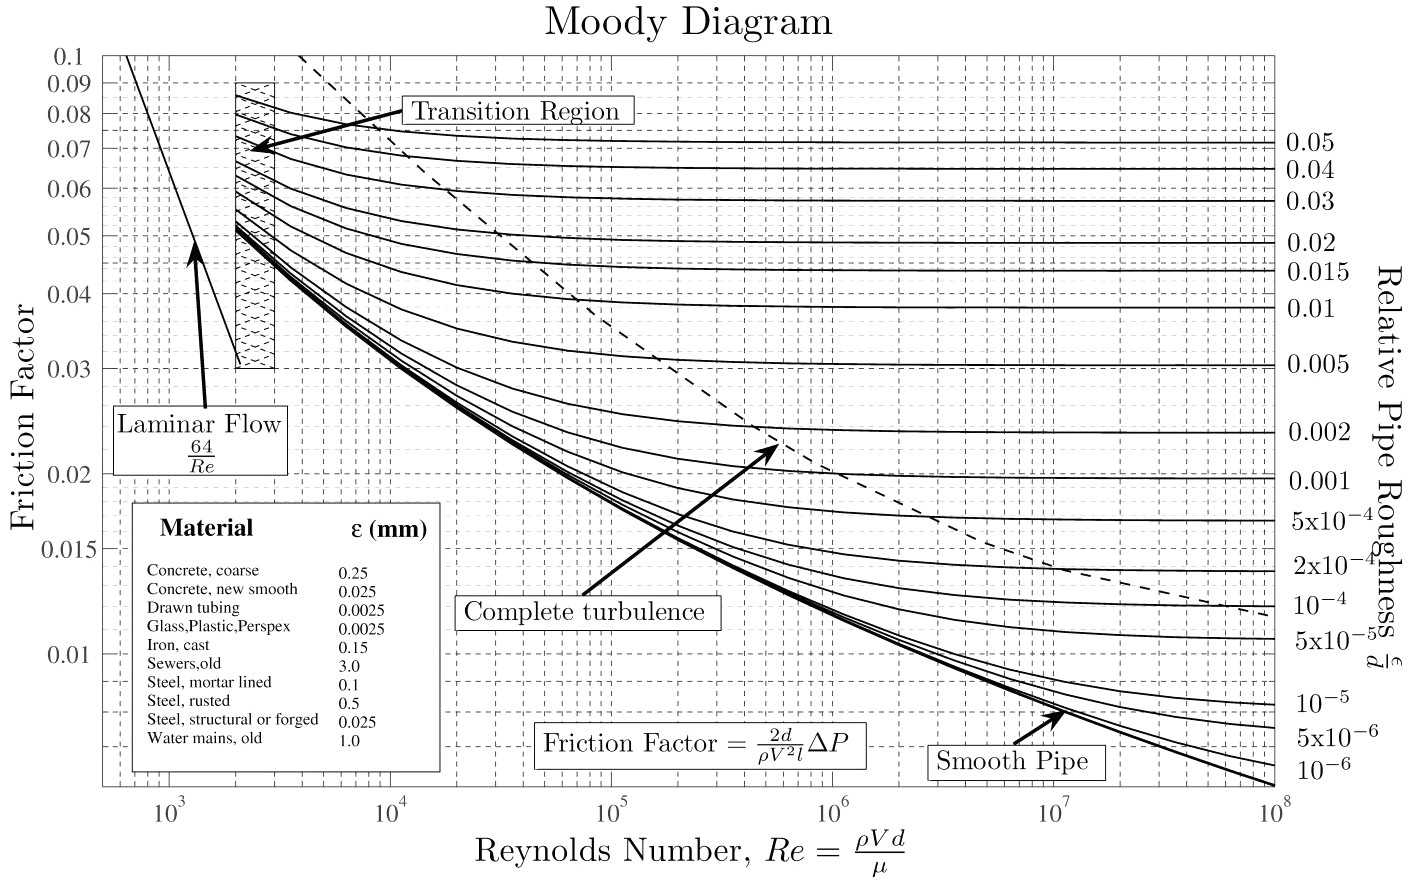
\includegraphics[clip,width=\linewidth]{figures/Moody_diagram}
\end{figure}

Laminar Power-Law fluid:
\begin{align*}
  \dot{V} = \frac{n\,\pi\,R^3}{3\,n+1} \left(\frac{R}{2\,k}\right)^{\frac{1}{n}} \left(-\frac{\Delta p}{L}\right)^{\frac{1}{n}}
\end{align*}
{\bf Two-Phase Flow:}\\*
Lockhart-Martinelli parameter:
\begin{align*}
  X^2=\frac{\Delta p_{liq.-only}}{\Delta p_{gas-only}}
\end{align*}
Pressure drop calculation:
\begin{align*}
  \Delta p_{two-phase} = \Phi^2_{liq.}\,\Delta p_{liq.-only} = \Phi^2_{gas}\,\Delta p_{gas-only}
\end{align*}
Chisholm's relation:
\begin{align*}
  \Phi^2_{gas} &= 1 + c\,X + X^2 &\\
  \Phi^2_{liq.} &= 1 + \frac{c}{X}+\frac{1}{X^2} &
  c &= \begin{cases}
    20& \text{turbulent liquid \& turbulent gas}\\
    12& \text{laminar liquid \& turbulent gas}\\
    10& \text{turbulent liquid \& laminar gas}\\
    5& \text{laminar liquid \& laminar gas}
  \end{cases}
\end{align*}
Farooqi and Richardson expression for liquid hold-up in co-current
flows of Newtonian fluids and air in horizontal pipes:
\begin{align*}
  h &=
  \begin{cases}
    0.186+0.0191\,X & 1 < X < 5\\
    0.143\,X^{0.42} & 5 < X < 50\\
    1/\left(0.97 + 19/X\right) & 50 < X < 500
  \end{cases}
\end{align*}

\begin{figure}[p!]%
  \begin{center}%
    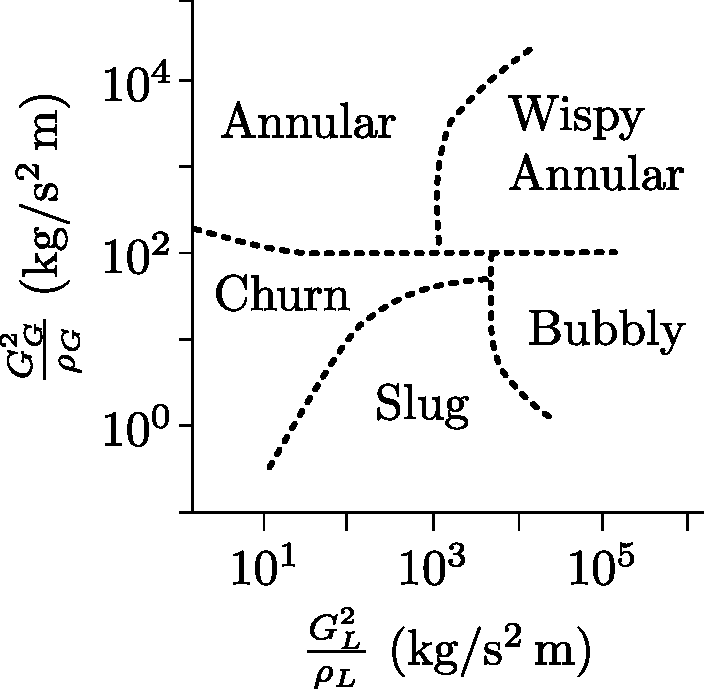
\includegraphics[width=0.65\textwidth,clip]{figures/Hewitt_Taylor}
  \end{center}
  \caption{Hewitt-Taylor flow pattern map for multiphase flows in
    vertical pipes.}
  \begin{center}%
    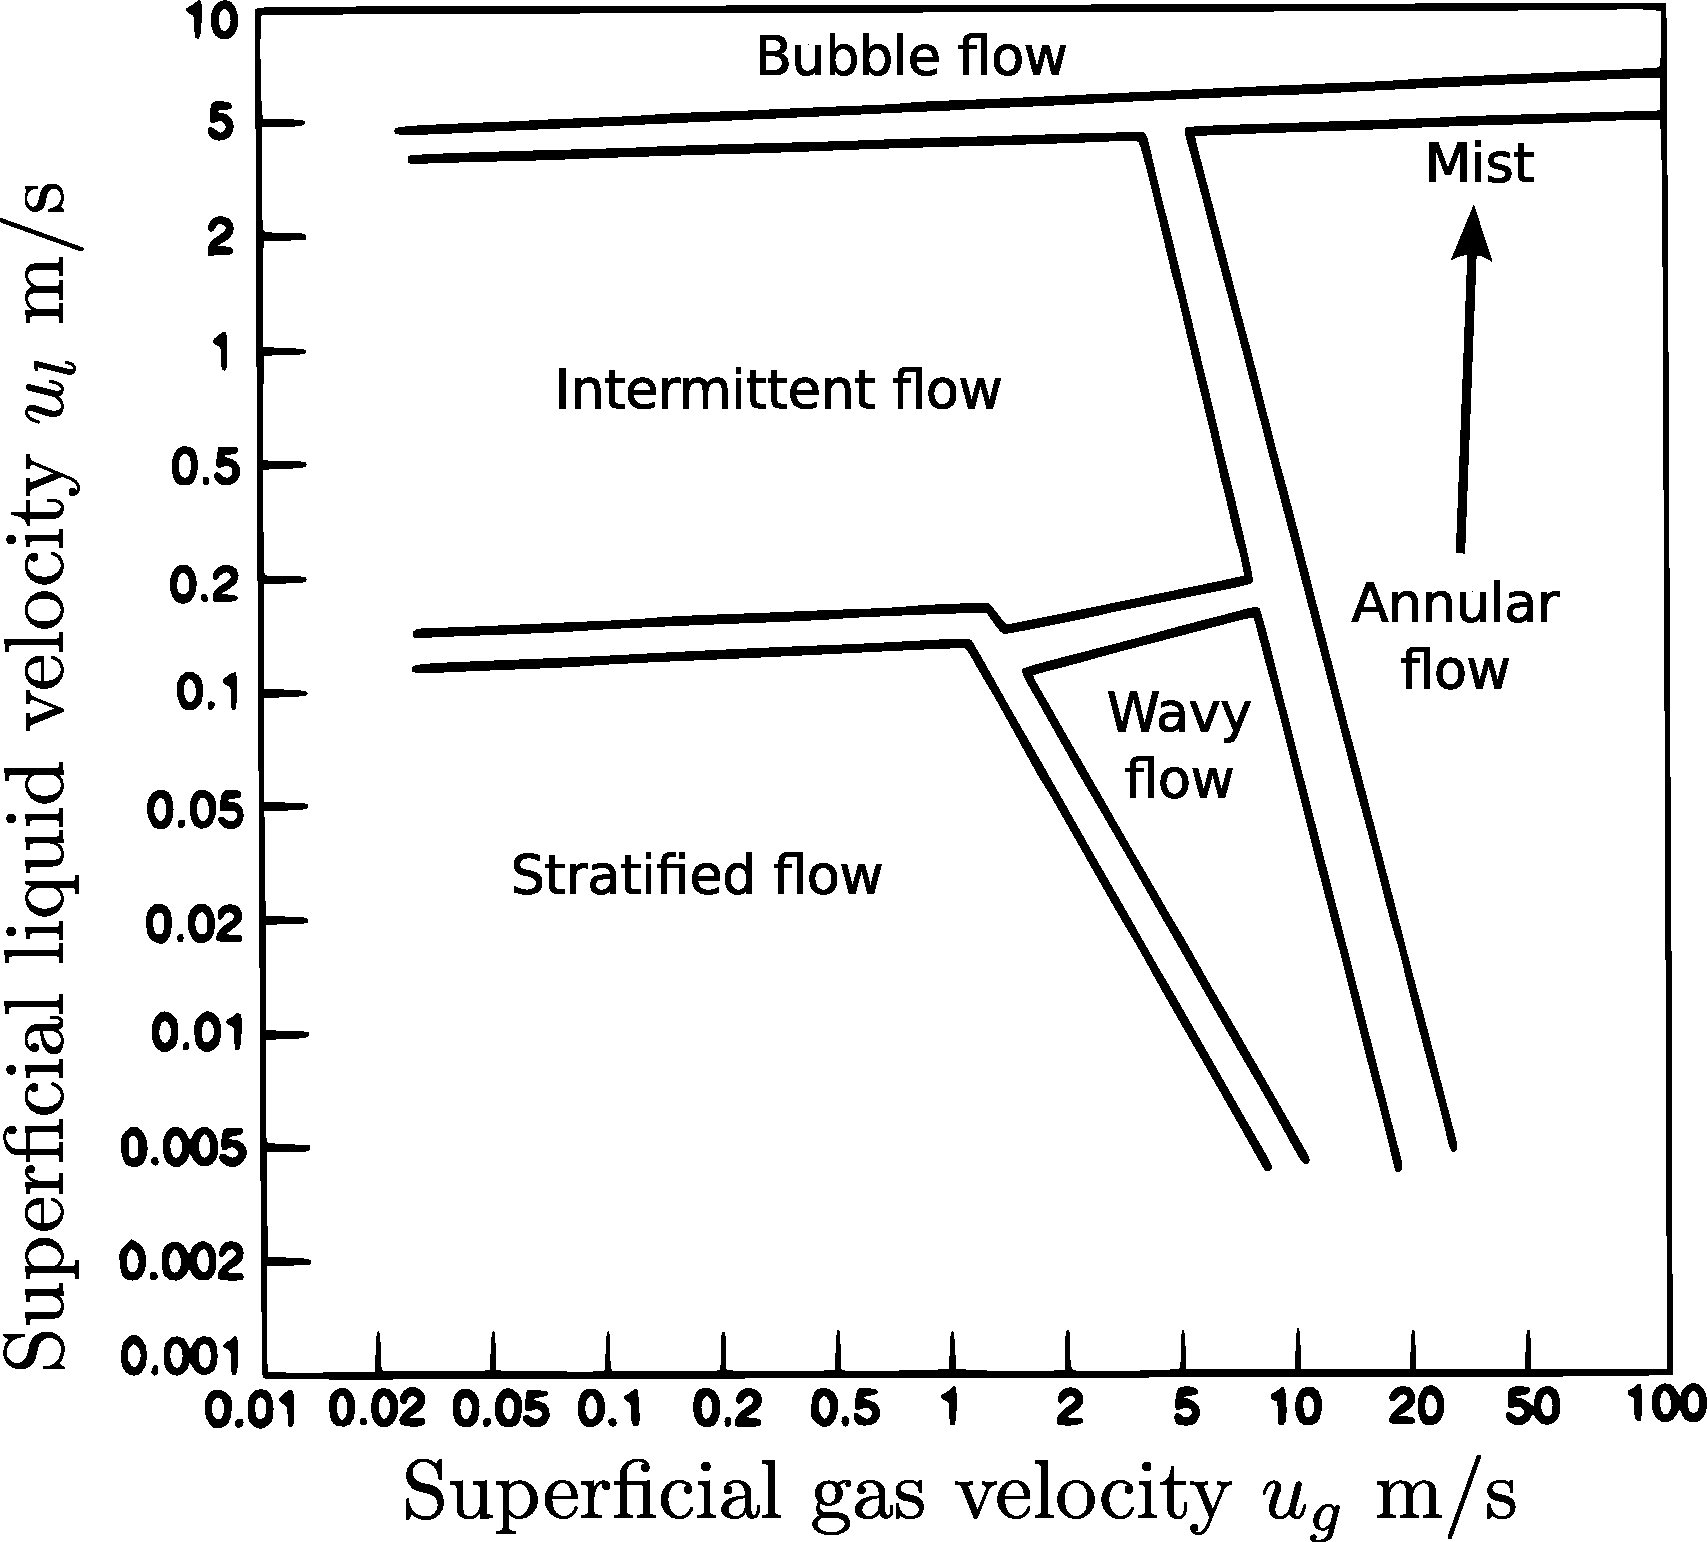
\includegraphics[width=0.65\textwidth,clip]{figures/Chhabra_richardson_flow_map}
  \end{center}
  \caption{Chhabra and Richardson flow pattern map for horizontal pipes.}
\end{figure}

\pagebreak[0]
{\bf Heat Transfer:}\\*
Stefan-Boltzmann constant $\sigma=5.6703\times10^{-8}$~W/m${}^2$~K${}^4$

{\bf Heat Transfer Dimensionless numbers:}
\begin{align*}
  \text{Nu} &= \frac{h\,L}{k} 
  &
  \text{Pr} &= \frac{\mu\,C_p}{k}
  &
  \text{Gr} &= \frac{g\,\beta
    \left(T_w - T_\infty\right)\,L^3}{\nu^2}
\end{align*}

{\bf Resistances}
\begin{align*}
  Q &= U_T\,A_T\,\Delta T = R_T^{-1}\,\Delta T & Q_{rad.}= \sigma\,\varepsilon\,A\left(T_\infty^4-T_w^4\right) = h_{rad.}\,A\left(T_\infty-T_w\right)
\end{align*}
\begin{center}
  \begin{tabular}{|r|c|c|c|c|}\hline
    & \multicolumn{3}{c|}{Conduction Shell Resistances} & Radiation\\
    & Rect. & Cyl. & Sph. & \\\hline
    & & & & \\
    $R$ & $\displaystyle\frac{X}{k\,A}$ & $\displaystyle\frac{\ln\left(R_{outer}/R_{inner}\right)}{2\,\pi\,L\,k}$ & $\displaystyle\frac{R_{inner}^{-1} - R_{outer}^{-1}}{4\,\pi\,k}$ & $\left[A\,\varepsilon\,\sigma\left(T_\infty^2+T_w^2\right)\left(T_\infty + T_w\right)\right]^{-1}$
    \\[5pt]\hline
  \end{tabular}
\end{center}

{\bf Natural Convection}
\begin{table}[h!]
  \begin{center}
    \begin{tabular}{|p{3cm}|p{3cm}|p{3cm}|}\hline
      $\text{Ra}=\text{Gr}\,\text{Pr}$ & $C$ & $m$\\\hline
      $< 10^{4}$ & 1.36 & 1/5\\
      $10^{4}$--$10^{9}$ & 0.59 & 1/4 \\
      $>10^{9}$ & 0.13 & 1/3\\\hline
    \end{tabular}
    \caption{\label{tab:conv}Natural convection coefficients for isothermal vertical
      plates in the empirical relation $\text{Nu}\approx C\left(\text{Gr}\,\text{Pr}\right)^m$.
      % The values are taken from Table~7-1 in ``Heat Transfer'' by J.\
      % P.\ Holman.
    }
  \end{center}
\end{table}

For isothermal vertical cylinders, the above expressions for
isothermal vertical plates may be used but must be scaled by a factor,
$F$:
\begin{align*}
  F = \begin{cases}
    1 & \text{for }\left(D/H\right) < 35\,\text{Gr}^{-1/4}_H
    \\
    1.3\left[H\,D^{-1}\,\text{Gr}_D^{-1}\right]^{1/4}+1 & \text{for }\left(D/H\right) \ge 35\,\text{Gr}^{-1/4}_H
  \end{cases}
\end{align*}
where $D$ is the diameter and $H$ is the height of the cylinder. The
subscript on $\text{Gr}$ indicates which length is to be used as the
critical length to calculate the Grashof number.

Churchill and Chu expression for natural convection from a
horizontal pipe:
\begin{align*}
  \text{Nu}^{1/2} &= 0.6 + 0.387
  \left\{\frac{\text{Gr}\,\text{Pr}}{\left[1 + \left(0.559 /
          \text{Pr}\right)^{9/16}\right]^{16/9}}\right\}^{1/6} &
  \text{for $10^{-5}<\text{Gr}\,\text{Pr}<10^{12}$}
\end{align*}%

{\bf Forced Convection:}\\*
Laminar flows:
\begin{align*}
  \text{Nu} \approx 0.332\,\text{Re}^{1/2}\,\text{Pr}^{1/3}
\end{align*}
Well-Developed turbulent flows in smooth pipes:
\begin{align*}
  \text{Nu} \approx \frac{(C_f/2)
    \text{Re}\,\text{Pr}}{1.07+12.7(C_f/2)^{1/2}\left(\text{Pr}^{2/3}
      -1\right)}\left(\frac{\mu_b}{\mu_w}\right)^{0.14}
\end{align*}

{\bf Boiling:}\\*
Forster-Zuber pool-boiling coefficient:
\begin{align*}
  h_{nb}=0.00122\frac{k_L^{0.79}\, C_{p,L}^{0.45}\, \rho_L^{0.49}}{\gamma^{0.5}\,\mu_L^{0.29}\,h_{fg}^{0.24}\,\rho_G^{0.24}}\left(T_w - T_{sat}\right)^{0.24}\left(p_w-p_{sat}\right)^{0.75}
\end{align*}

Mostinski correlations: 
\begin{align*}
  h_{nb} &= 0.104\,p_c^{0.69}\,q^{0.7}\left[1.8\left(\frac{p}{p_c}\right)^{0.17}+4\left(\frac{p}{p_c}\right)^{1.2}+10\left(\frac{p}{p_c}\right)^{10}\right]\\
  q_c &=
  3.67\times10^4\,p_c\left(\frac{p}{p_c}\right)^{0.35}\left[1-\frac{p}{p_c}\right]^{0.9}
\end{align*}
({\bf Note}: for the Mostinski correlations, the pressures are in units of bar)\\*
{\bf Condensing:}\\*
Horizontal pipes
\begin{align*}
  h = 0.72
  \left(\frac{k^3\,\rho^2\,g_x\,E_{latent}}{D\,\mu\,\left(T_w-T_\infty\right)}\right)^{1/4}
\end{align*}

{\bf Lumped capacitance method:}\\*
\begin{align*}
  \text{Bi} &= \frac{h\,L_c}{\kappa} & \\
  L_c &= 
  V/A & \text{for $\text{Bi}<0.1$}
\end{align*}

{\bf 1-D Transient Heat Conduction:}\\*
\begin{align*}
   Fo = \frac{\alpha \Delta t}{\left(\Delta x\right)^{2}}
\end{align*}


\begin{align*}
   \theta_{\text{wall}} = \frac{T(x,t)-T_{\infty}}{T_{i}-T_{\infty}}= A_{1}e^{-\lambda_{1}^{2}\tau}\cos{\left(\frac{\lambda_{1}x}{L}\right)},\;\;\;\;\; \theta_{\text{cyl}} = \frac{T(r,t)-T_{\infty}}{T_{i}-T_{\infty}}= A_{1}e^{-\lambda_{1}^{2}\tau}\mathbf{J_{0}}\left(\frac{\lambda_{1}r}{r_{0}}\right)
\end{align*}

\begin{align*}
   \theta_{\text{sph}} = \frac{T(r,t)-T_{\infty}}{T_{i}-T_{\infty}}= A_{1}e^{-\lambda_{1}^{2}\tau}\frac{\sin{\left(\frac{\lambda_{1}r}{r_{0}}\right)}}{\frac{\lambda_{1}r}{r_{0}}}
\end{align*}


\begin{align*}
   \left(\frac{\mathcal{Q}}{\mathcal{Q}_{\text{max}}}\right)_{\text{wall}} = 1 - \theta_{0,\text{wall}}\frac{\sin{\lambda_{1}}}{\lambda_{1}},\;\;\left(\frac{\mathcal{Q}}{\mathcal{Q}_{\text{max}}}\right)_{\text{cyl}} = 1- 2\theta_{0,\text{cyl}}\frac{\mathbf{J_{1}}}{\lambda_{1}}
\end{align*}

\begin{align*}
    \left(\frac{\mathcal{Q}}{\mathcal{Q}_{\text{max}}}\right)_{\text{sph}} = 1 - 3\theta_{0,\text{sph}}\frac{\sin{\lambda_{1}}-\lambda_{1}\cos{\lambda_{1}}}{\lambda_{1}^{3}}
\end{align*}

\begin{figure}[h!]%
  \begin{center}%
    \includegraphics[width=0.7\textwidth,clip]{figures/BaselFunctionTable}
  \end{center}
  \caption{Coefficients for the 1D transient equations.}
\end{figure}


\pagebreak[0]

{\bf Overall Heat Transfer Coefficient:}\\*
\begin{align*}
  \dot{\mathcal{Q}} =  \frac{\Delta T}{\mathcal{R}} = U A \Delta T  = U_{i}A_{i}\Delta T = U_{o}A_{o}\Delta T
\end{align*}

\begin{align*}
  \mathcal{R} = R_{i} + R_{\text{wall}} + R_{o} = \frac{1}{h_{i}A_{i}} + \frac{\ln{D_{o}/D_{i}}}{2\pi \kappa L} + \frac{1}{h_{o}A_{o}} 
\end{align*}

{\bf Fouling Factor:}*
\begin{align*}
   \mathcal{R} = \frac{1}{h_{i}A_{i}} + \frac{R_{\text{f,i}}}{A_{i}} + R_{\text{wall}} + \frac{R_{\text{f,o}}}{A_{o}} + \frac{1}{h_{o}A_{o}}
\end{align*}

{\bf LMTD Method:}\\*
\begin{align*}
   \dot{\mathcal{Q}} = U A_{s} \Delta T_{\text{lm}}\;\text{ with }\;  \Delta T_{\text{lm}} = \frac{\left(T_{\text{hot,out}} - T_{\text{cold,out}}\right)-\left(T_{\text{hot,in}} - T_{\text{cold,in}}\right)}{\ln{\left(\frac{T_{\text{hot,out}} - T_{\text{cold,out}}}{T_{\text{hot,in}} - T_{\text{cold,in}}}\right)}}.
\end{align*}

\begin{figure}[h!]%
  \begin{center}%
    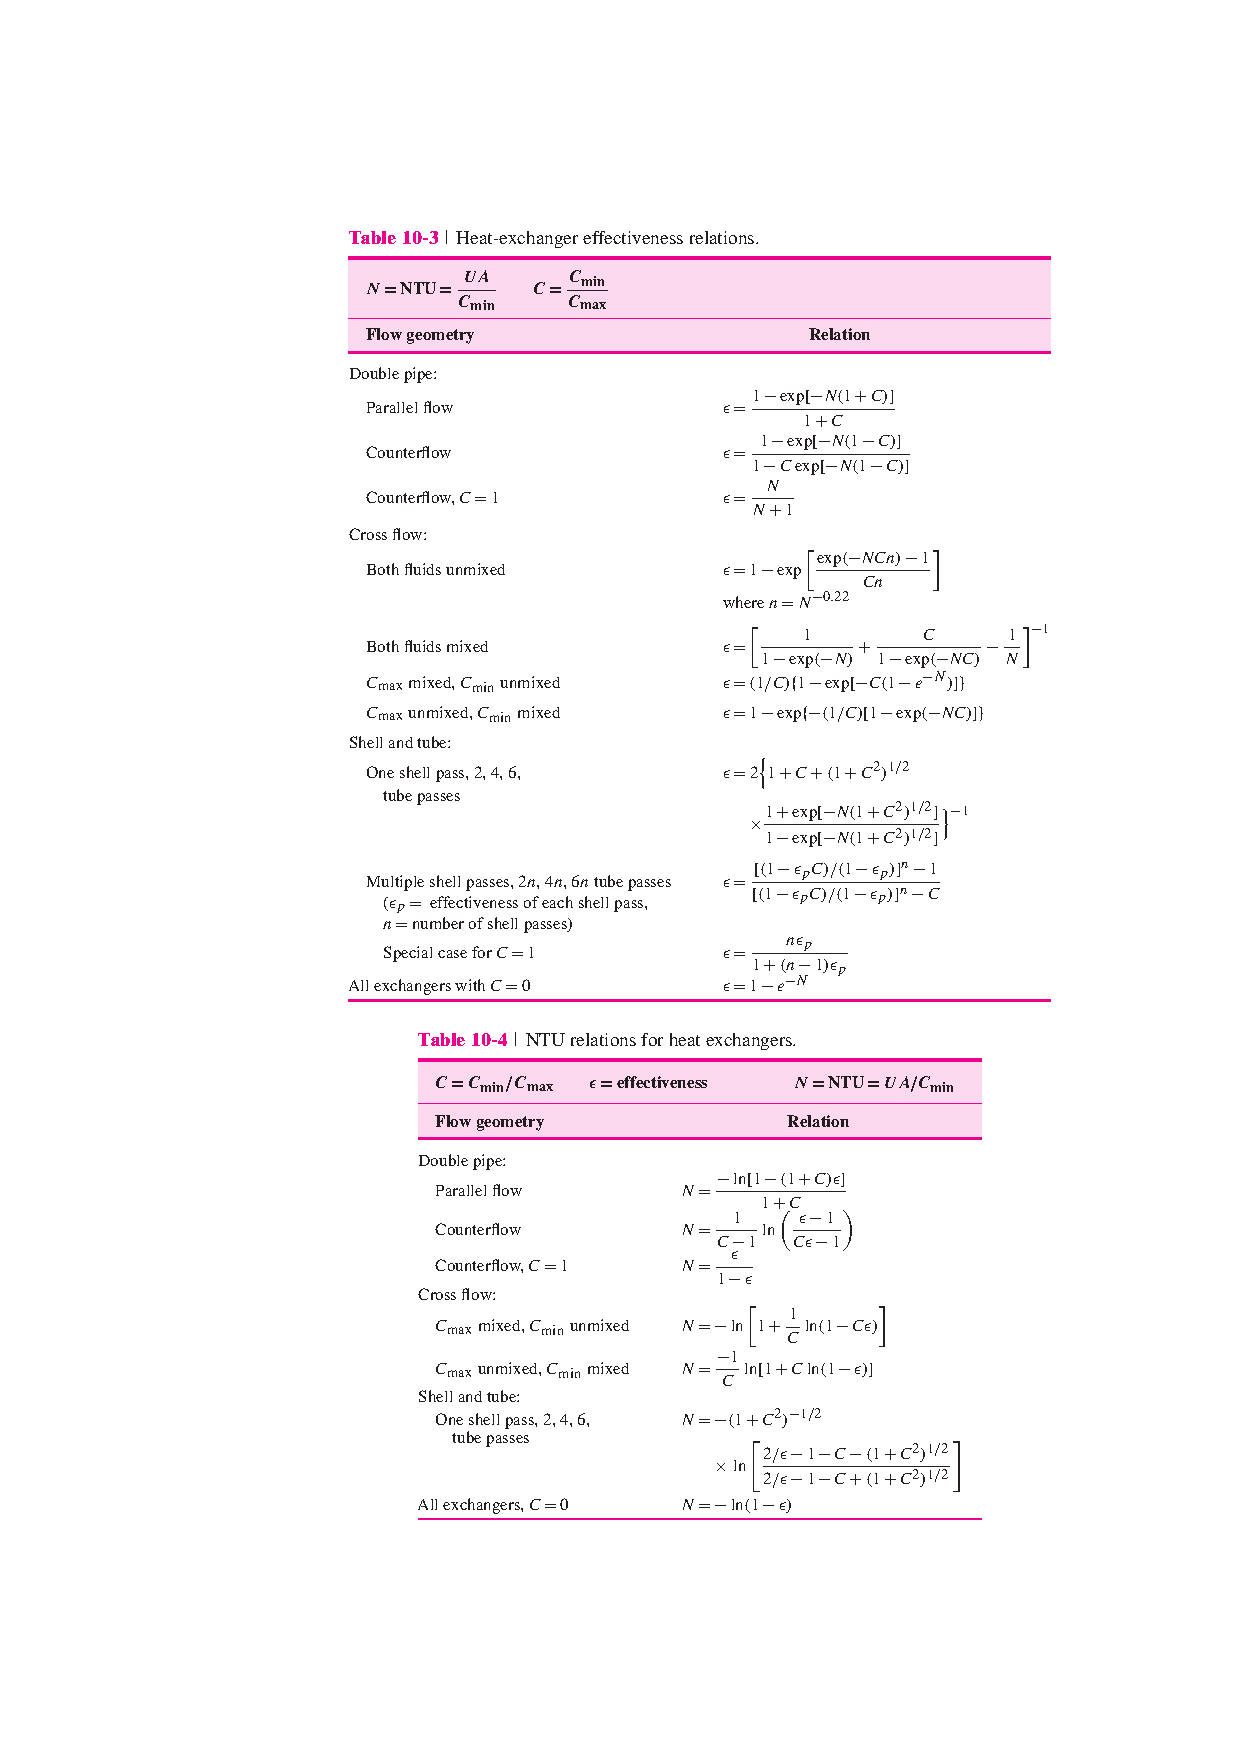
\includegraphics[width=0.8\textwidth,clip]{figures/NTU}
  \end{center}
  \caption{NTU relations}
\end{figure}


\pagebreak[0]
{\bf Diffusion Dimensionless Numbers}\\*
\begin{align*}
  \text{Sc} &= \frac{\mu}{\rho\,D_{AB}} & \text{Le} &= \frac{k}{\rho\,C_p\,D_{AB}}
\end{align*}
\pagebreak[0]
{\bf Diffusion}\\*
General expression for the flux:
\begin{align*}
  \bm{N}_{A} = \bm{J}_A + x_A \sum_B \bm{N}_B
\end{align*}
Fick's law:
\begin{align*}
  \bm{J}_{A} = - D_{AB}\,\nabla C_A
\end{align*}
Stefan's law:
\begin{align*}
  N_{s,r} = -D \frac{c}{1-x}\frac{\partial x}{\partial r}
\end{align*}
{\bf Misc}\\*
\begin{align*}
  P\,V &= n\,R\,T & 
  R&\approx8.314598~\text{J K}^{-1}\text{ mol}^{-1} 
\end{align*}
\end{datasheet}

% \includepdf{BaselFunctionTable.pdf}
\paperend
\end{document}
